
%% bare_jrnl.tex
%% V1.3
%% 2007/01/11
%% by Michael Shell
%% see http://www.michaelshell.org/
%% for current contact information.
%%
%% This is a skeleton file demonstrating the use of IEEEtran.cls
%% (requires IEEEtran.cls version 1.7 or later) with an IEEE journal paper.
%%
%% Support sites:
%% http://www.michaelshell.org/tex/ieeetran/
%% http://www.ctan.org/tex-archive/macros/latex/contrib/IEEEtran/
%% and
%% http://www.ieee.org/



% *** Authors should verify (and, if needed, correct) their LaTeX system  ***
% *** with the testflow diagnostic prior to trusting their LaTeX platform ***
% *** with production work. IEEE's font choices can trigger bugs that do  ***
% *** not appear when using other class files.                            ***
% The testflow support page is at:
% http://www.michaelshell.org/tex/testflow/


%%*************************************************************************
%% Legal Notice:
%% This code is offered as-is without any warranty either expressed or
%% implied; without even the implied warranty of MERCHANTABILITY or
%% FITNESS FOR A PARTICULAR PURPOSE! 
%% User assumes all risk.
%% In no event shall IEEE or any contributor to this code be liable for
%% any damages or losses, including, but not limited to, incidental,
%% consequential, or any other damages, resulting from the use or misuse
%% of any information contained here.
%%
%% All comments are the opinions of their respective authors and are not
%% necessarily endorsed by the IEEE.
%%
%% This work is distributed under the LaTeX Project Public License (LPPL)
%% ( http://www.latex-project.org/ ) version 1.3, and may be freely used,
%% distributed and modified. A copy of the LPPL, version 1.3, is included
%% in the base LaTeX documentation of all distributions of LaTeX released
%% 2003/12/01 or later.
%% Retain all contribution notices and credits.
%% ** Modified files should be clearly indicated as such, including  **
%% ** renaming them and changing author support contact information. **
%%
%% File list of work: IEEEtran.cls, IEEEtran_HOWTO.pdf, bare_adv.tex,
%%                    bare_conf.tex, bare_jrnl.tex, bare_jrnl_compsoc.tex
%%*************************************************************************

% Note that the a4paper option is mainly intended so that authors in
% countries using A4 can easily print to A4 and see how their papers will
% look in print - the typesetting of the document will not typically be
% affected with changes in paper size (but the bottom and side margins will).
% Use the testflow package mentioned above to verify correct handling of
% both paper sizes by the user's LaTeX system.
%
% Also note that the "draftcls" or "draftclsnofoot", not "draft", option
% should be used if it is desired that the figures are to be displayed in
% draft mode.
%
\documentclass[journal,twoside]{IEEEtran}
\usepackage{blindtext}
\usepackage{graphicx}
\usepackage{textcomp}
\usepackage{subfig}
\usepackage{multirow}
\usepackage{authblk}
\usepackage{amsmath}

% Some very useful LaTeX packages include:
% (uncomment the ones you want to load)


% *** MISC UTILITY PACKAGES ***
%
%\usepackage{ifpdf}
% Heiko Oberdiek's ifpdf.sty is very useful if you need conditional
% compilation based on whether the output is pdf or dvi.
% usage:
% \ifpdf
%   % pdf code
% \else
%   % dvi code
% \fi
% The latest version of ifpdf.sty can be obtained from:
% http://www.ctan.org/tex-archive/macros/latex/contrib/oberdiek/
% Also, note that IEEEtran.cls V1.7 and later provides a builtin
% \ifCLASSINFOpdf conditional that works the same way.
% When switching from latex to pdflatex and vice-versa, the compiler may
% have to be run twice to clear warning/error messages.






% *** CITATION PACKAGES ***
%
%\usepackage{cite}
% cite.sty was written by Donald Arseneau
% V1.6 and later of IEEEtran pre-defines the format of the cite.sty package
% \cite{} output to follow that of IEEE. Loading the cite package will
% result in citation numbers being automatically sorted and properly
% "compressed/ranged". e.g., [1], [9], [2], [7], [5], [6] without using
% cite.sty will become [1], [2], [5]--[7], [9] using cite.sty. cite.sty's
% \cite will automatically add leading space, if needed. Use cite.sty's
% noadjust option (cite.sty V3.8 and later) if you want to turn this off.
% cite.sty is already installed on most LaTeX systems. Be sure and use
% version 4.0 (2003-05-27) and later if using hyperref.sty. cite.sty does
% not currently provide for hyperlinked citations.
% The latest version can be obtained at:
% http://www.ctan.org/tex-archive/macros/latex/contrib/cite/
% The documentation is contained in the cite.sty file itself.






% *** GRAPHICS RELATED PACKAGES ***
%
\ifCLASSINFOpdf
  % \usepackage[pdftex]{graphicx}
  % declare the path(s) where your graphic files are
  % \graphicspath{{../pdf/}{../jpeg/}}
  % and their extensions so you won't have to specify these with
  % every instance of \includegraphics
  % \DeclareGraphicsExtensions{.pdf,.jpeg,.png}
\else
  % or other class option (dvipsone, dvipdf, if not using dvips). graphicx
  % will default to the driver specified in the system graphics.cfg if no
  % driver is specified.
  % \usepackage[dvips]{graphicx}
  % declare the path(s) where your graphic files are
  % \graphicspath{{../eps/}}
  % and their extensions so you won't have to specify these with
  % every instance of \includegraphics
  % \DeclareGraphicsExtensions{.eps}
\fi
% graphicx was written by David Carlisle and Sebastian Rahtz. It is
% required if you want graphics, photos, etc. graphicx.sty is already
% installed on most LaTeX systems. The latest version and documentation can
% be obtained at: 
% http://www.ctan.org/tex-archive/macros/latex/required/graphics/
% Another good source of documentation is "Using Imported Graphics in
% LaTeX2e" by Keith Reckdahl which can be found as epslatex.ps or
% epslatex.pdf at: http://www.ctan.org/tex-archive/info/
%
% latex, and pdflatex in dvi mode, support graphics in encapsulated
% postscript (.eps) format. pdflatex in pdf mode supports graphics
% in .pdf, .jpeg, .png and .mps (metapost) formats. Users should ensure
% that all non-photo figures use a vector format (.eps, .pdf, .mps) and
% not a bitmapped formats (.jpeg, .png). IEEE frowns on bitmapped formats
% which can result in "jaggedy"/blurry rendering of lines and letters as
% well as large increases in file sizes.
%
% You can find documentation about the pdfTeX application at:
% http://www.tug.org/applications/pdftex





% *** MATH PACKAGES ***
%
%\usepackage[cmex10]{amsmath}
% A popular package from the American Mathematical Society that provides
% many useful and powerful commands for dealing with mathematics. If using
% it, be sure to load this package with the cmex10 option to ensure that
% only type 1 fonts will utilized at all point sizes. Without this option,
% it is possible that some math symbols, particularly those within
% footnotes, will be rendered in bitmap form which will result in a
% document that can not be IEEE Xplore compliant!
%
% Also, note that the amsmath package sets \interdisplaylinepenalty to 10000
% thus preventing page breaks from occurring within multiline equations. Use:
%\interdisplaylinepenalty=2500
% after loading amsmath to restore such page breaks as IEEEtran.cls normally
% does. amsmath.sty is already installed on most LaTeX systems. The latest
% version and documentation can be obtained at:
% http://www.ctan.org/tex-archive/macros/latex/required/amslatex/math/





% *** SPECIALIZED LIST PACKAGES ***
%
%\usepackage{algorithmic}
% algorithmic.sty was written by Peter Williams and Rogerio Brito.
% This package provides an algorithmic environment fo describing algorithms.
% You can use the algorithmic environment in-text or within a figure
% environment to provide for a floating algorithm. Do NOT use the algorithm
% floating environment provided by algorithm.sty (by the same authors) or
% algorithm2e.sty (by Christophe Fiorio) as IEEE does not use dedicated
% algorithm float types and packages that provide these will not provide
% correct IEEE style captions. The latest version and documentation of
% algorithmic.sty can be obtained at:
% http://www.ctan.org/tex-archive/macros/latex/contrib/algorithms/
% There is also a support site at:
% http://algorithms.berlios.de/index.html
% Also of interest may be the (relatively newer and more customizable)
% algorithmicx.sty package by Szasz Janos:
% http://www.ctan.org/tex-archive/macros/latex/contrib/algorithmicx/




% *** ALIGNMENT PACKAGES ***
%
%\usepackage{array}
% Frank Mittelbach's and David Carlisle's array.sty patches and improves
% the standard LaTeX2e array and tabular environments to provide better
% appearance and additional user controls. As the default LaTeX2e table
% generation code is lacking to the point of almost being broken with
% respect to the quality of the end results, all users are strongly
% advised to use an enhanced (at the very least that provided by array.sty)
% set of table tools. array.sty is already installed on most systems. The
% latest version and documentation can be obtained at:
% http://www.ctan.org/tex-archive/macros/latex/required/tools/


%\usepackage{mdwmath}
%\usepackage{mdwtab}
% Also highly recommended is Mark Wooding's extremely powerful MDW tools,
% especially mdwmath.sty and mdwtab.sty which are used to format equations
% and tables, respectively. The MDWtools set is already installed on most
% LaTeX systems. The lastest version and documentation is available at:
% http://www.ctan.org/tex-archive/macros/latex/contrib/mdwtools/


% IEEEtran contains the IEEEeqnarray family of commands that can be used to
% generate multiline equations as well as matrices, tables, etc., of high
% quality.


%\usepackage{eqparbox}
% Also of notable interest is Scott Pakin's eqparbox package for creating
% (automatically sized) equal width boxes - aka "natural width parboxes".
% Available at:
% http://www.ctan.org/tex-archive/macros/latex/contrib/eqparbox/





% *** SUBFIGURE PACKAGES ***
%\usepackage[tight,footnotesize]{subfigure}
% subfigure.sty was written by Steven Douglas Cochran. This package makes it
% easy to put subfigures in your figures. e.g., "Figure 1a and 1b". For IEEE
% work, it is a good idea to load it with the tight package option to reduce
% the amount of white space around the subfigures. subfigure.sty is already
% installed on most LaTeX systems. The latest version and documentation can
% be obtained at:
% http://www.ctan.org/tex-archive/obsolete/macros/latex/contrib/subfigure/
% subfigure.sty has been superceeded by subfig.sty.



%\usepackage[caption=false]{caption}
%\usepackage[font=footnotesize]{subfig}
% subfig.sty, also written by Steven Douglas Cochran, is the modern
% replacement for subfigure.sty. However, subfig.sty requires and
% automatically loads Axel Sommerfeldt's caption.sty which will override
% IEEEtran.cls handling of captions and this will result in nonIEEE style
% figure/table captions. To prevent this problem, be sure and preload
% caption.sty with its "caption=false" package option. This is will preserve
% IEEEtran.cls handing of captions. Version 1.3 (2005/06/28) and later 
% (recommended due to many improvements over 1.2) of subfig.sty supports
% the caption=false option directly:
%\usepackage[caption=false,font=footnotesize]{subfig}
%
% The latest version and documentation can be obtained at:
% http://www.ctan.org/tex-archive/macros/latex/contrib/subfig/
% The latest version and documentation of caption.sty can be obtained at:
% http://www.ctan.org/tex-archive/macros/latex/contrib/caption/




% *** FLOAT PACKAGES ***
%
%\usepackage{fixltx2e}
% fixltx2e, the successor to the earlier fix2col.sty, was written by
% Frank Mittelbach and David Carlisle. This package corrects a few problems
% in the LaTeX2e kernel, the most notable of which is that in current
% LaTeX2e releases, the ordering of single and double column floats is not
% guaranteed to be preserved. Thus, an unpatched LaTeX2e can allow a
% single column figure to be placed prior to an earlier double column
% figure. The latest version and documentation can be found at:
% http://www.ctan.org/tex-archive/macros/latex/base/



%\usepackage{stfloats}
% stfloats.sty was written by Sigitas Tolusis. This package gives LaTeX2e
% the ability to do double column floats at the bottom of the page as well
% as the top. (e.g., "\begin{figure*}[!b]" is not normally possible in
% LaTeX2e). It also provides a command:
%\fnbelowfloat
% to enable the placement of footnotes below bottom floats (the standard
% LaTeX2e kernel puts them above bottom floats). This is an invasive package
% which rewrites many portions of the LaTeX2e float routines. It may not work
% with other packages that modify the LaTeX2e float routines. The latest
% version and documentation can be obtained at:
% http://www.ctan.org/tex-archive/macros/latex/contrib/sttools/
% Documentation is contained in the stfloats.sty comments as well as in the
% presfull.pdf file. Do not use the stfloats baselinefloat ability as IEEE
% does not allow \baselineskip to stretch. Authors submitting work to the
% IEEE should note that IEEE rarely uses double column equations and
% that authors should try to avoid such use. Do not be tempted to use the
% cuted.sty or midfloat.sty packages (also by Sigitas Tolusis) as IEEE does
% not format its papers in such ways.


%\ifCLASSOPTIONcaptionsoff
%  \usepackage[nomarkers]{endfloat}
% \let\MYoriglatexcaption\caption
% \renewcommand{\caption}[2][\relax]{\MYoriglatexcaption[#2]{#2}}
%\fi
% endfloat.sty was written by James Darrell McCauley and Jeff Goldberg.
% This package may be useful when used in conjunction with IEEEtran.cls'
% captionsoff option. Some IEEE journals/societies require that submissions
% have lists of figures/tables at the end of the paper and that
% figures/tables without any captions are placed on a page by themselves at
% the end of the document. If needed, the draftcls IEEEtran class option or
% \CLASSINPUTbaselinestretch interface can be used to increase the line
% spacing as well. Be sure and use the nomarkers option of endfloat to
% prevent endfloat from "marking" where the figures would have been placed
% in the text. The two hack lines of code above are a slight modification of
% that suggested by in the endfloat docs (section 8.3.1) to ensure that
% the full captions always appear in the list of figures/tables - even if
% the user used the short optional argument of \caption[]{}.
% IEEE papers do not typically make use of \caption[]'s optional argument,
% so this should not be an issue. A similar trick can be used to disable
% captions of packages such as subfig.sty that lack options to turn off
% the subcaptions:
% For subfig.sty:
% \let\MYorigsubfloat\subfloat
% \renewcommand{\subfloat}[2][\relax]{\MYorigsubfloat[]{#2}}
% For subfigure.sty:
% \let\MYorigsubfigure\subfigure
% \renewcommand{\subfigure}[2][\relax]{\MYorigsubfigure[]{#2}}
% However, the above trick will not work if both optional arguments of
% the \subfloat/subfig command are used. Furthermore, there needs to be a
% description of each subfigure *somewhere* and endfloat does not add
% subfigure captions to its list of figures. Thus, the best approach is to
% avoid the use of subfigure captions (many IEEE journals avoid them anyway)
% and instead reference/explain all the subfigures within the main caption.
% The latest version of endfloat.sty and its documentation can obtained at:
% http://www.ctan.org/tex-archive/macros/latex/contrib/endfloat/
%
% The IEEEtran \ifCLASSOPTIONcaptionsoff conditional can also be used
% later in the document, say, to conditionally put the References on a 
% page by themselves.





% *** PDF, URL AND HYPERLINK PACKAGES ***
%
%\usepackage{url}
% url.sty was written by Donald Arseneau. It provides better support for
% handling and breaking URLs. url.sty is already installed on most LaTeX
% systems. The latest version can be obtained at:
% http://www.ctan.org/tex-archive/macros/latex/contrib/misc/
% Read the url.sty source comments for usage information. Basically,
% \url{my_url_here}.





% *** Do not adjust lengths that control margins, column widths, etc. ***
% *** Do not use packages that alter fonts (such as pslatex).         ***
% There should be no need to do such things with IEEEtran.cls V1.6 and later.
% (Unless specifically asked to do so by the journal or conference you plan
% to submit to, of course. )


% correct bad hyphenation here
%\hyphenation{op-tical net-works semi-conduc-tor}


\begin{document}
%
% paper title
% can use linebreaks \\ within to get better formatting as desired
\title{Autonomous Navigation of a Mobile Robot in Indoor Environments}
%
%
% author names and IEEE memberships
% note positions of commas and nonbreaking spaces ( ~ ) LaTeX will not break
% a structure at a ~ so this keeps an author's name from being broken across
% two lines.
% use \thanks{} to gain access to the first footnote area
% a separate \thanks must be used for each paragraph as LaTeX2e's \thanks
% was not built to handle multiple paragraphs
%

\author{\IEEEauthorblockN{Bimal Paneru, Niraj Basnet, Sagar Shrestha, Rabin Giri and
Dinesh Baniya Kshetri}
\IEEEauthorblockA{ \\Department of Electronics and Computer Engineering\\
Central Campus, Institute of Engineering, Tribhuvan University\\}}

% note the % following the last \IEEEmembership and also \thanks - 
% these prevent an unwanted space from occurring between the last author name
% and the end of the author line. i.e., if you had this:
% 
% \author{....lastname \thanks{...} \thanks{...} }
%                     ^------------^------------^----Do not want these spaces!
%
% a space would be appended to the last name and could cause every name on that
% line to be shifted left slightly. This is one of those "LaTeX things". For
% instance, "\textbf{A} \textbf{B}" will typeset as "A B" not "AB". To get
% "AB" then you have to do: "\textbf{A}\textbf{B}"
% \thanks is no different in this regard, so shield the last } of each \thanks
% that ends a line with a % and do not let a space in before the next \thanks.
% Spaces after \IEEEmembership other than the last one are OK (and needed) as
% you are supposed to have spaces between the names. For what it is worth,
% this is a minor point as most people would not even notice if the said evil
% space somehow managed to creep in.



% The paper headers
\markboth{Zerone Scholar,~Vol.~1, No.~1, November~2016}%
{Paneru \MakeLowercase{\textit{et al.}}: Autonomous Navigation of a Mobile Robot in Indoor Environments}
% The only time the second header will appear is for the odd numbered pages
% after the title page when using the twoside option.
% 
% *** Note that you probably will NOT want to include the author's ***
% *** name in the headers of peer review papers.                   ***
% You can use \ifCLASSOPTIONpeerreview for conditional compilation here if
% you desire.




% If you want to put a publisher's ID mark on the page you can do it like
% this:
%\IEEEpubid{0000--0000/00\$00.00~\copyright~2007 IEEE}
% Remember, if you use this you must call \IEEEpubidadjcol in the second
% column for its text to clear the IEEEpubid mark.



% use for special paper notices
%\IEEEspecialpapernotice{(Invited Paper)}




% make the title area
\maketitle

\begin{abstract}
%\boldmath
This paper presents the use of probabilistic algorithms in a differential drive robot for totally autonomous navigation in indoor environment. The robot is capable of building map of its environment and global localization in the map thus built. The robot then performs path planning to compute an optimal path towards the goal location. We make use of LiDAR for mapping and localization, and a Microsoft Kinect is used in addition to detect obstacles not falling in the plane of LiDAR.
\end{abstract}
% IEEEtran.cls defaults to using nonbold math in the Abstract.
% This preserves the distinction between vectors and scalars. However,
% if the journal you are submitting to favors bold math in the abstract,
% then you can use LaTeX's standard command \boldmath at the very start
% of the abstract to achieve this. Many IEEE journals frown on math
% in the abstract anyway.

% Note that keywords are not normally used for peerreview papers.
\begin{IEEEkeywords}
Navigation, LiDAR, Mapping, Localization, Robot.
\end{IEEEkeywords}


% For peer review papers, you can put extra information on the cover
% page as needed:
% \ifCLASSOPTIONpeerreview
% \begin{center} \bfseries EDICS Category: 3-BBND \end{center}
% \fi
%
% For peerreview papers, this IEEEtran command inserts a page break and
% creates the second title. It will be ignored for other modes.
\IEEEpeerreviewmaketitle

\section{Introduction}
\noindent Growing interest in navigation systems is due to the possibility of their use in a wide range of environments and conditions. Fully automatic indoor navigation system has been successfully implemented in robotic restaurant, cleaning robots, warehouse robots. Autonomuos navigation can be broken down into three major tasks - localization, mapping and path planning. The result of navigation is executed by motion control system that implements PID control [1]. The inputs to the position and orientation estimation are sensor data acquired from gyroscope, digital compass and encoders. Complementary filter [2] and Kalman filter [3] are two widely used techniques for sensor fusion. Since Kalman filter gives a better result [4], though computationally complex, we use Kalman filter over complementary. \par\noindent Commonly used localization approaches include Monte Carlo Localization(MCL) [5] which is a particle filter based method, Extended Kalman Filter(EKF) [6], and Adaptive Monte Carlo Localization(AMCL) [7] which uses adaptive resampling technique to account for particle deprivation problem. Mapping is accomplished through occupancy grid mapping that uses LiDAR scan data to build a two dimensional map of the environment [8].The map thus built is a metric grid of binary random variables each of whose value corresponds to the presence or absence of obstacle at that point. \par\noindent Given a known robot location, an optimal or suboptimal path can be computed towards a desired goal in the map provided that a possible path exists. Graph search techniques are more popular than other algorithms such as potential field [9] because of the simplicity in dealing with nodes and branches represented by cells and their location in the map. Such graph based techniques include A* [10], D* [11], Dijkstra’s search [12]. 
\begin{figure}[h]
\centering
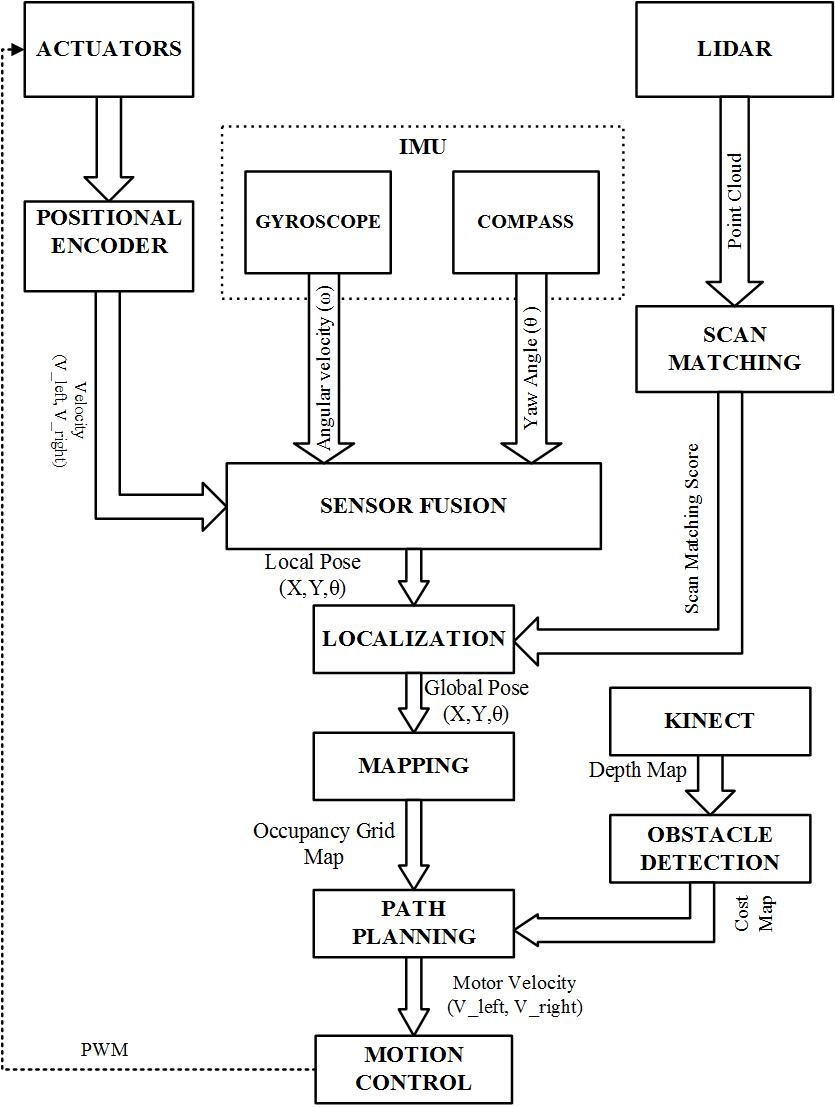
\includegraphics[scale=.3]{1.jpg}
\DeclareGraphicsExtensions.
\caption{System Block Diagram}
\end{figure}
\par\noindent Correct execution of total path planned using these algorithms is an important issue. Moreover, global plan might not always be realizable given the dynamic constraints of the robot. To ensure correct and efficient execution of such plan, local planner is required. Local planner does not completely comply with global plan but finds a suitable compromise between global and local plan. Local planner, basically, takes a segment of the global plan and outputs required velocities for the motors. Dynamic window approach is one of such planners developed to support navigation at greater speed [13]. A complete solution for navigation is found out by the combination of appropriate algorithms to accomplish each task of navigation. Fig.1 shows our approach for navigation of a differential drive robot. IMU and encoder data are fused to obtain an estimate of the local position. Scan matching of LiDAR data with the available map assigns a score to each local pose computed for particles in monte carlo localization. This results in an estimate of the global pose that is used both for mapping and subsequently for path planning. The result of path planning assigns motor velocities to motion control unit which runs PID control to give appropriate PWM signals to the motors.

\section{Sensor Fusion Using Kalman Filter}
\noindent Kalman filter is a Gaussian filter, meaning it assumes that its beliefs (which in our case is going to be the gyroscope measurement) can be represented by multivariate normal distribution. It is probably the best studied technique for Bayesian Filter implementation. The kalman filtering process can be broken down into two major steps, the prediction stage and the measurement update.
\subsection{The Prediction Stage}
\noindent It calculates the next state prediction. The next state probability $p(x_t|u_t, x_{t-1})$ must be a linear function in its arguments with added Gaussian noise. The equation representing this function is
\begin{equation}
x_{t|t-1} = F_t x_{t-1|t-1} + B_t u_t
\end{equation} 
\begin{equation}
P_{t|t-1} = F_t P_{t-1|t−1} P_{t-1|t-1} F_t^T + Q_t
\end{equation} 
\par\noindent where,\newline
$x_{t|t-1}$ is the predicted state from previous state $x_{t-1|t-1}$.\newline
$F_t$ and $B_t$ are the state transition matrix and input transformation matrix respectively.\newline
$P_{t|t-1}$ is the variance associated with the prediction $x_{t|t-1}$ of an unknown true value of the state.\newline
$Q_t$ is a multivariate Gaussian to model the noise associated with the transition.\newline

\subsection{Measurement Update}
\noindent The measurement probability must also be linear in its arguments, with added Gaussian noise. This stage is represented by a set of equations that are as follows:
\begin{equation}
x_{t|t} = x_{t|t-1} + K_t(z_t-H_t x_{t|t-1})
\end{equation} 
\begin{equation}
P_{t|t} = P_{t|t-1} - K_t H_t P_{t|t-1}
\end{equation} 
\begin{equation}
K_t = P_{t|t-1} H_t^T (H_t P_{t|t-1} H_t^T + R_t)-1
\end{equation} 
\par\noindent where,\newline
$z_t$ is the measurement and can be modeled as: $z_t = H_t x_t + R_t$
\par\noindent In this equation $H_t$ is the transformation matrix to transform state space into measurement space. And $R_t$ is the measurement noise covariance matrix.
\par\noindent The primary parameter from all this computation is the Kalman gain Kt which determines the amount of trust to be put into the measurement and prediction in order to calculate the posterior. The posterior at this state becomes the prior of the next state and so on. 
\begin{figure}[h]
\centering
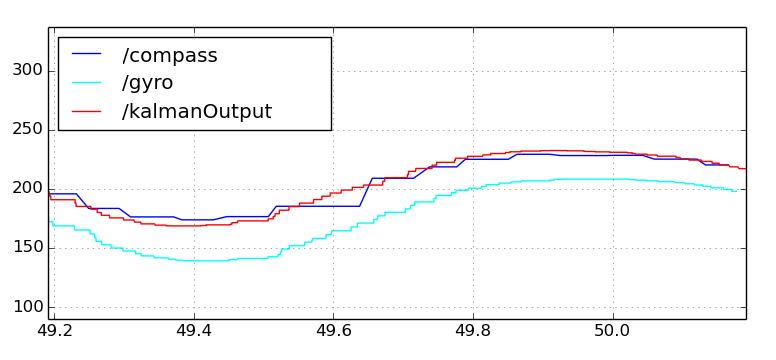
\includegraphics[scale=.3]{2.jpg}
\DeclareGraphicsExtensions.
\caption{Sensor Fusion Using Kalman Filter}
\end{figure}
\par\noindent Clearly in our case, the two inputs are gyroscope and digital compass. The gyroscope data replaces the input $u_t$. And the measurement z is given by compass data.
\begin{equation}
\binom{x_{angle}}{x_{bias}}_{t|t-1} = \binom{1~~-dt}{0~~~~~~1} \binom{x_{angle}}{x_{bias}}_{t-1|t-1} + \binom{dt}{0} u_t
\end{equation}
\section{Localization Using AMCL}
\noindent Adaptive Monte Carlo localization (AMCL) is one of the most popular localization algorithms, which represents estimated pose by particles. It is a variant of implementation of particle filter and an improvised version of MCL, to localize the robot in given world space of map. The algorithm estimates the position and orientation of a robot in the given map as it moves and senses the environment. The algorithm can be used for global localization problem. It uses a particle filter to represent the distribution of likely states, with each particle representing a possible state, i.e. a hypothesis of for robot’s position. 
\par\noindent Initially, the algorithm starts with a uniform random distribution of particles over the configuration space, meaning the robot makes an assumption that it can be at any point in given space. So,the initial belief bel(x0) is obtained by randomly
generating M such particles from the prior distribution p(x0), and assigning the uniform importance to each particle. For initial set of uniformly distributed particles, for each particle the motion model (odometry model) is computed to find new pose for particles. So actuation command is simulated for every particles no matter where they are and what direction they are pointing. The sensor measurement model is then applied to determine the importance weight of that particle. Then, it randomly draws new particles from the previous belief, with probability proportional to weight of particle. Particles which were consistent with sensor readings are more likely to be chosen and particles which are inconsistent with
sensor readings are rarely picked. As such, particles converge towards a better estimate of the robot’s state. After some interval of time, the particle sets approximate the correct posterior and localization becomes successful. It is easy to implement, and tends to work well across a broad range of localization problems which MCL fails to address like robot kidnapping problem where particle deprivation is the most common issue.
\begin{figure}[h]
\centering
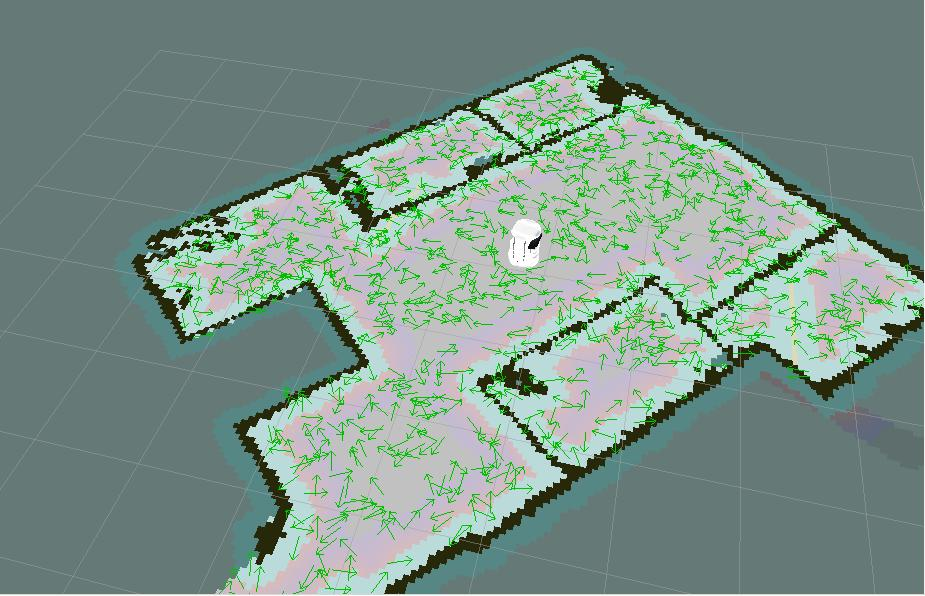
\includegraphics[scale=.27]{3.jpg}
\DeclareGraphicsExtensions.
\caption{Random Particle Injection Before Resampling}
\end{figure}
\par\noindent To solve robot kidnapping problem and global localization problems of MCL, the original MCL is augmented with adaptive sampling stage which adapts the number of particles according to the error in posterior estimate. It is accomplished by using the KullbackLeibler divergence (KLD) method and since the improvisation is adaptive in nature, the modified MCL is known as Adaptive MCL. The notion of this method is to add random particles to the particle sets and this addition of random particles can be justified mathematically by assuming that the robot might get kidnapped with a small probability , thereby generating a fraction of random states in the motion model. This addition is determined by the degree of localization accuracy through short term and long term measurement likelihoods. The re-sampling condition used in this algorithm requires that $0\leq\alpha_{slow}\ll\alpha_{fast}$, where parameters $\alpha_{slow}$, and $\alpha_{fast}$, are decay rates used in the exponential filters for estimating the long-term and short-term measurement likelihoods respectively. A random sample is dded based on the probability max(0 : 0; 1.0 - $\frac{\omega_{fast}}{\omega_{slow}}$). If the short-term likelihood approximates the long-term likelihood, re-sampling occurs normally without any extra injection of particles.But if the short-term likelihood is worse than the long-term one, then the probability of addition of random samples increases accordingly. Thus, a sudden decay in measurement likelihood results in an increased number of particles in resampling step and number of particles adapt to this change in measurement likelihood. Therefore, in practice, AMCL can consistently outperform and converge faster than classic MCL for localization of robot.

\section{Occupancy Grid Mapping}
\noindent Occupancy grid mapping is a probabilistic technique to build a map that correctly represents the environment from sensor measurements done after successful localization. The fundamental idea of the algorithm is to represent the environment in two dimensional grid of evenly space cells weighted by binary random variables that determine the presence of obstacle. The algorithm computes approximate posterior estimates for these random variables to correctly represent robot’s operating environments.
\begin{figure}[h]
\centering
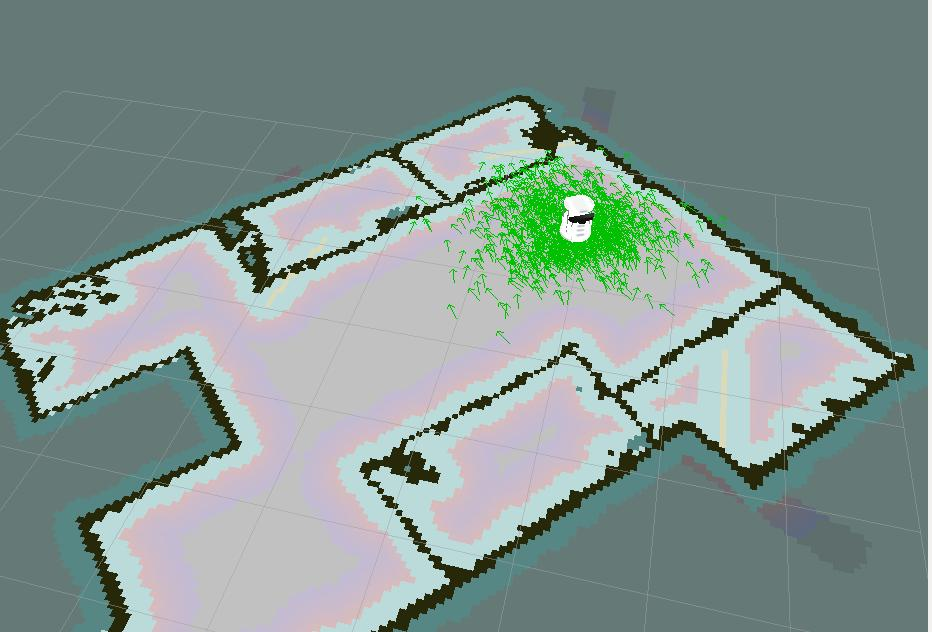
\includegraphics[scale=.27]{4.jpg}
\DeclareGraphicsExtensions.
\caption{Converged Particles After Resampling}
\end{figure}
\begin{figure}[h]
\centering
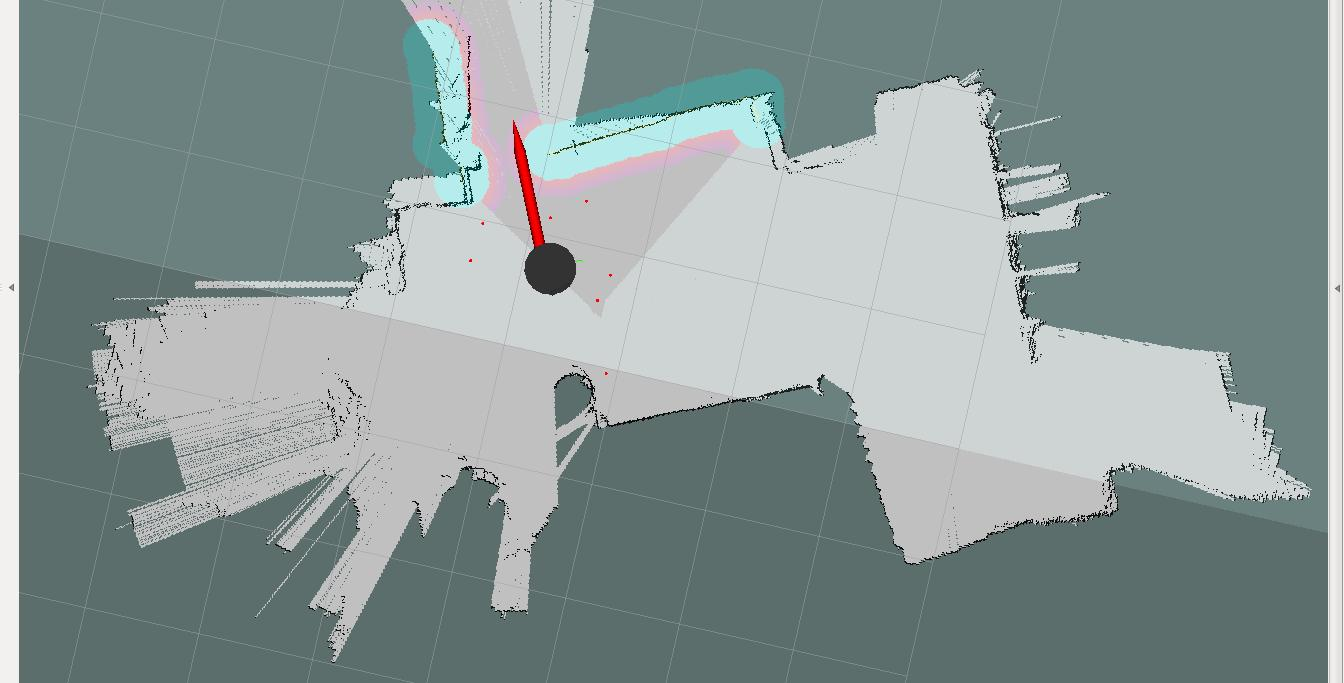
\includegraphics[scale=.19]{5.jpg}
\DeclareGraphicsExtensions.
\caption{Occupancy Grid Mapping Using LiDAR}
\end{figure}
\par\noindent The environment is represented metric grids of variables that correspond the occupancy of the environment. The occupancy of grid is represented by three color values: gray for unexplored space, white for free space and black for occupied space.A suitable threshold value is used to transition between these three states.It is particularly suitable for robot with range sensors like LiDAR whose value can be directly raytraced to determine occupancy of desired cell. Robot is allowed to travel only in free space denoted by white region and hence it provides reference for finding paths in unoccupied space preventing potential collision risks. The probability of occupancy of each grid cell m given the measurements $z_1...z_T$ is given as
$$p(m|z_1...z_t)$$
\par\noindent We calculate the log-odds as: \newline
\begin{equation}
l^t_{x,y} = log\frac{p(m_{x,y}|z_t)}{1-p(m_{x,y}|z_t)}+ log\frac{1-p(m_{x,y})}{p(m_{x,y})}+l^{t-1}_{x,y} 
\end{equation} 
\begin{equation}
l^0_{x,y} = log\frac{p(m_{x,y})}{1-p(m_{x,y})}
\end{equation} 
\section{Path Planning}
\noindent The path planning stage is divided into two parts - global and local planner. Global planner plans the total path from the robot location to goal location. This path is further split into several smaller paths to be executed in the local planner. Local planner ensures correct navigation to each intermediate goal points.

\subsection{Global Planner}
\noindent Global Planner uses A* search algorithm. Each cell in the map is a node in the graph. A* reduces the number of nodes to be expanded from source to goal. In order to determine the likelihood of the node to fall on optimal path, it uses a heuristic function in addition to evaluation function. g(n) is the cost function that gives the distance of node n from the source. Heuristic function h(n) in our case gives the minimum distance of node n from the goal. So the evaluation function of a node is the sum of actual cost from node to source and optimistic estimate(minimum distance) of the cost from node to goal as in equation 9.
\begin{equation}
f(n) = g(n) + h(n)
\end{equation}
\subsection{Local Planner}
\noindent The local planner implements dynamic window approach which has been proved to be very efficient for high speed obstacle avoidance. In dynamic window approach the kinematics of the robot is taken into account by considering only those velocities that can be attained in the next time frame given the acceleration constraints and time period. Given the current robot velocity, a dynamic window is computed that contains all admissible tuples (v,w). This approach is implemented by the maximization of the objective function. The objective function incorporates the following:
\begin{equation}
O = a.target(v, w) + b.velocity(v, w) + c.clearance(v, w)
\end{equation}
\par 1) Target heading, the measure of progress towards the goal location supporting the direction directly towards the goal location 
\par 2) Clearance, the distance to the closest obstacle on the trajectory
\par 3) Velocity, the forward velocity of the robot supporting fast movements

\section{Results}
\noindent All the tasks of navigation were successfully accomplished with afore mentioned techniques. The robot was able navigate to a position in a pre-built map by globally localizing itself at first, planning an optimal path and executing motion commands thus generated. Fig.6 shows the formation of occupancy grid map from odometry and laserscan data.The 3d point cloud obtained from kinect also matches the result obtained from laserscan data.
\par\noindent The black pixels as a whole represent some form of obstacle like wall,door,desks and benches. As previously explained, white zone represents free space where robot can travel freely and grey zone represents unexplored region which the robot has still left to incorporate in its map. Fig.7 shows the complete 2D occupancy map generated of a classroom. We can visualize the general floor plan of this room from this map.Each pixel represents an area of 0.05 ∗ 0.05cm2 .The resolution of map can be further reduced to 0.25 cm, however it increase runtime memory and computation overhead.
\begin{figure}[h!]
\centering
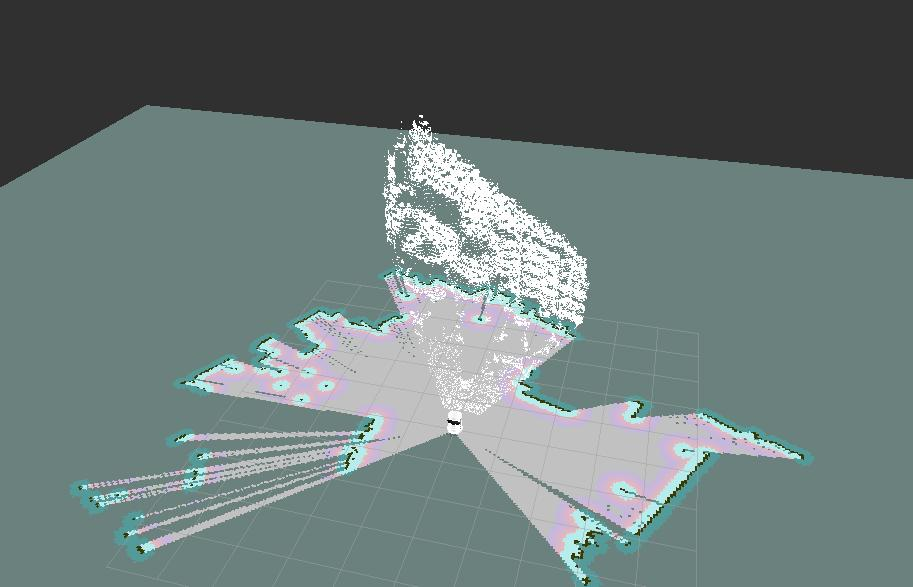
\includegraphics[scale=.27]{6.jpg}
\DeclareGraphicsExtensions.
\caption{Mapping From LiDAR Laserscan and Odometry}
\end{figure}
\begin{figure}[h!]
\centering
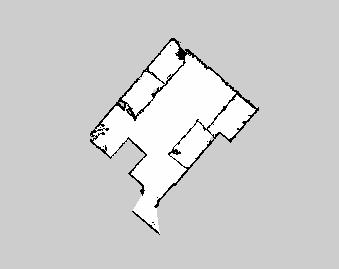
\includegraphics[scale=.73]{7.jpg}
\DeclareGraphicsExtensions.
\caption{Complete Map Built of a Classroom}
\end{figure}
\begin{figure}[h!]
\centering
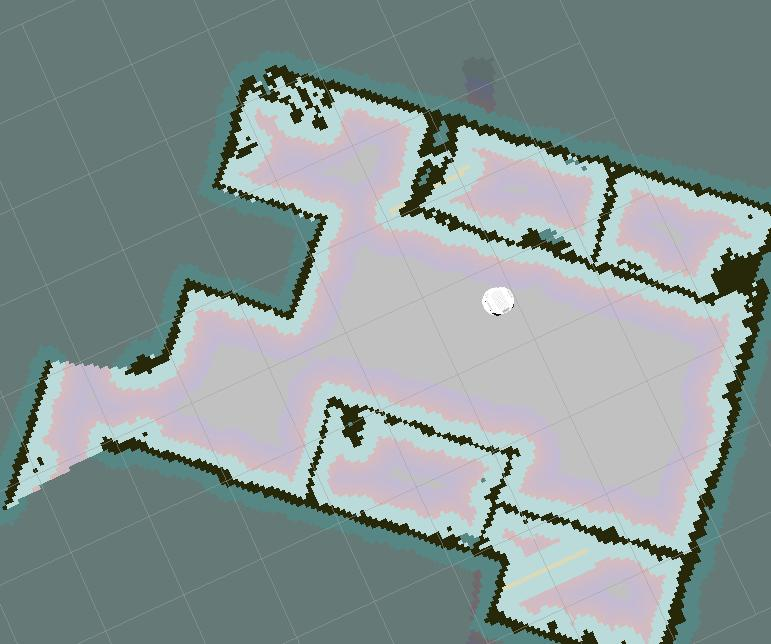
\includegraphics[scale=.32]{8.jpg}
\DeclareGraphicsExtensions.
\caption{Global Costmap With Obstacle Layer of 0.3m}
\end{figure}
\par\noindent Fig.8 shows the region in the whole map where the robot is fit to travel without any risk of collision. The cost of traveling to particular region around the obstacles is increased, hence constituting global costmap. The obstacle layer represented in the map by black pixel figures is further inflated to a certain distance(in our case 0.5m) depending upon the base surface area of robot, so that robot can plan a safe path around these potential collision prone regions. 
\begin{figure}[h]
\centering
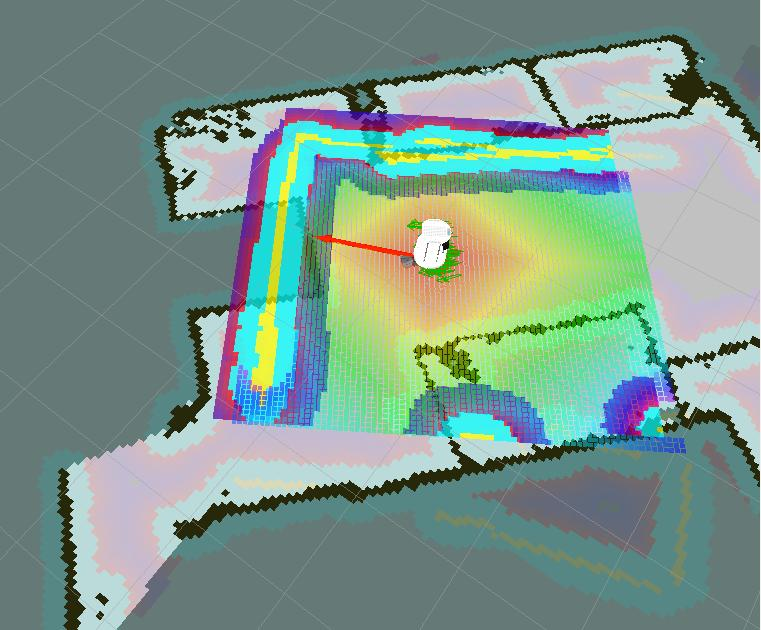
\includegraphics[scale=.27]{9.jpg}
\DeclareGraphicsExtensions.
\caption{Local Costmap With Obstacle Layer of 0.5m With Cost Decay 10}
\end{figure}
\par\noindent Fig.9 shows the local region around the robot in the global map, where robot continuously monitors static as well as dynamic obstacles to plan immediate course of action. The local costmap is a rectangular window of 3 by 3 meters. As seen in the figure, the nearby obstacles are inflated even beyond the global obstacle layer with certain cost decay i.e.,cost decreases gradually with distance from any obstacle.
\begin{figure}[h]
\centering
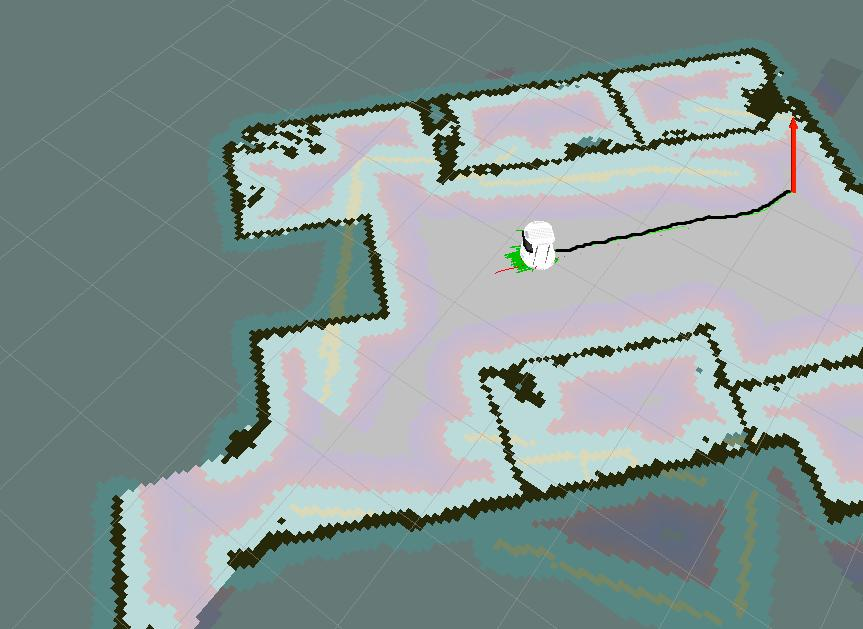
\includegraphics[scale=.27]{10.jpg}
\DeclareGraphicsExtensions.
\caption{Global Path Planning}
\end{figure}
\par\noindent Fig.10 is global path computed from the robot’s current location to the goal. The path is represented by a black curve joining the robot’s position to goal location. The global path is computed every second from robot’s current location to account for the error in navigation.  
\begin{figure}[h]
\centering
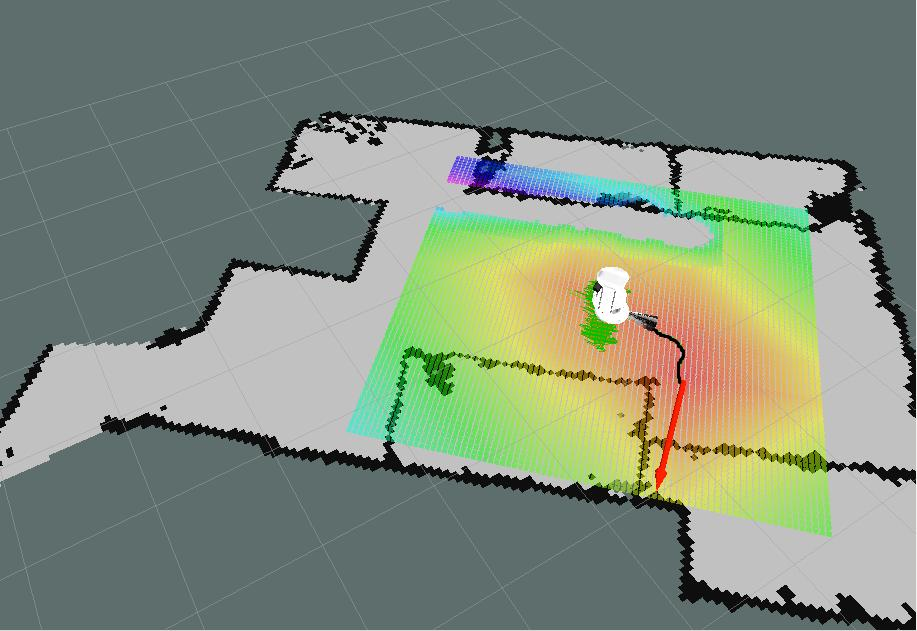
\includegraphics[scale=.27]{11.jpg}
\DeclareGraphicsExtensions.
\caption{Local Path Planning}
\end{figure}
\par\noindent Fig.11 is the local plan for the robot. Short lines protruding from the robot’s location is the set of admissible velocities and the black cure is the global path. Objective function for each plan is computed and maximized in order to choose a suitable velocity.

\section{Conclusion}
\noindent We were able to successfully navigate the robot in simulation and in real hardwares with some self built ROS nodes and some packages already existing in the ROS community. Range sensor produced better result during localization than depth camera. So mapping and localization were done using LiDAR. But since LiDAR scans on a single plane and many objects are completely or partially missed on its plane, Kinect depth camera was used to gain appropriate estimate of the obstacle’s occupancy. Use of depth camera in addition to range sensor has enabled us to effectively locate obstacles
and navigate clear off them. To sum up the results, sensor fusion of IMU data for orientation was accomplished with 2 degree tolerance. Localization with MCL was done with 500 particles and in the adaptive mode it could increase to as many as 2000 particles. Mapping was done with grid size 2048 * 2048 and scale: 1 pixel equivalent to 0.05 meters. And finally, path planning resulted in less than 0.2 meters deviation on final location. Research of algorithms and their comparisons were made thoroughly during the development of the robot.


% needed in second column of first page if using \IEEEpubid
%\IEEEpubidadjcol

% An example of a floating figure using the graphicx package.
% Note that \label must occur AFTER (or within) \caption.
% For figures, \caption should occur after the \includegraphics.
% Note that IEEEtran v1.7 and later has special internal code that
% is designed to preserve the operation of \label within \caption
% even when the captionsoff option is in effect. However, because
% of issues like this, it may be the safest practice to put all your
% \label just after \caption rather than within \caption{}.
%
% Reminder: the "draftcls" or "draftclsnofoot", not "draft", class
% option should be used if it is desired that the figures are to be
% displayed while in draft mode.
%
%\begin{figure}[!t]
%\centering
%\includegraphics[width=2.5in]{myfigure}
% where an .eps filename suffix will be assumed under latex, 
% and a .pdf suffix will be assumed for pdflatex; or what has been declared
% via \DeclareGraphicsExtensions.
%\caption{Simulation Results}
%\label{fig_sim}
%\end{figure}

% Note that IEEE typically puts floats only at the top, even when this
% results in a large percentage of a column being occupied by floats.


% An example of a double column floating figure using two subfigures.
% (The subfig.sty package must be loaded for this to work.)
% The subfigure \label commands are set within each subfloat command, the
% \label for the overall figure must come after \caption.
% \hfil must be used as a separator to get equal spacing.
% The subfigure.sty package works much the same way, except \subfigure is
% used instead of \subfloat.
%
%\begin{figure*}[!t]
%\centerline{\subfloat[Case I]\includegraphics[width=2.5in]{subfigcase1}%
%\label{fig_first_case}}
%\hfil
%\subfloat[Case II]{\includegraphics[width=2.5in]{subfigcase2}%
%\label{fig_second_case}}}
%\caption{Simulation results}
%\label{fig_sim}
%\end{figure*}
%
% Note that often IEEE papers with subfigures do not employ subfigure
% captions (using the optional argument to \subfloat), but instead will
% reference/describe all of them (a), (b), etc., within the main caption.


% An example of a floating table. Note that, for IEEE style tables, the 
% \caption command should come BEFORE the table. Table text will default to
% \footnotesize as IEEE normally uses this smaller font for tables.
% The \label must come after \caption as always.
%
%\begin{table}[!t]
%% increase table row spacing, adjust to taste
%\renewcommand{\arraystretch}{1.3}
% if using array.sty, it might be a good idea to tweak the value of
% \extrarowheight as needed to properly center the text within the cells
%\caption{An Example of a Table}
%\label{table_example}
%\centering
%% Some packages, such as MDW tools, offer better commands for making tables
%% than the plain LaTeX2e tabular which is used here.
%\begin{tabular}{|c||c|}
%\hline
%One & Two\\
%\hline
%Three & Four\\
%\hline
%\end{tabular}
%\end{table}


% Note that IEEE does not put floats in the very first column - or typically
% anywhere on the first page for that matter. Also, in-text middle ("here")
% positioning is not used. Most IEEE journals use top floats exclusively.
% Note that, LaTeX2e, unlike IEEE journals, places footnotes above bottom
% floats. This can be corrected via the \fnbelowfloat command of the
% stfloats package.




% if have a single appendix:
%\appendix[Proof of the Zonklar Equations]
% or
%\appendix  % for no appendix heading
% do not use \section anymore after \appendix, only \section*
% is possibly needed

% use appendices with more than one appendix
% then use \section to start each appendix
% you must declare a \section before using any
% \subsection or using \label (\appendices by itself
% starts a section numbered zero.)

%\appendices
%\section{Something Goes Here, but what?}
%Some text for the appendix.

% use section* for acknowledgement

% Can use something like this to put references on a page
% by themselves when using endfloat and the captionsoff option.
\ifCLASSOPTIONcaptionsoff
  \newpage
\fi



% trigger a \newpage just before the given reference
% number - used to balance the columns on the last page
% adjust value as needed - may need to be readjusted if
% the document is modified later
%\IEEEtriggeratref{8}
% The "triggered" command can be changed if desired:
%\IEEEtriggercmd{\enlargethispage{-5in}}

% references section

% can use a bibliography generated by BibTeX as a .bbl file
% BibTeX documentation can be easily obtained at:
% http://www.ctan.org/tex-archive/biblio/bibtex/contrib/doc/
% The IEEEtran BibTeX style support page is at:
% http://www.michaelshell.org/tex/ieeetran/bibtex/
%\bibliographystyle{IEEEtran}
% argument is your BibTeX string definitions and bibliography database(s)
%\bibliography{IEEEabrv,../bib/paper}
%
% <OR> manually copy in the resultant .bbl file
% set second argument of \begin to the number of references
% (used to reserve space for the reference number labels box)
\begin{thebibliography}{1}
%\bibitem{IEEEhowto:kopka}
%H.~Kopka and P.~W. Daly, \emph{A Guide to \LaTeX}, 3rd~ed. Harlow, England: Addison-Wesley, 1999.
\bibitem{}
M. Araki, “Pid control,” Control systems, robotics and automation, vol. 2, pp. 1-23, 2002.
\bibitem{}
P. C. Glasser, “An introduction to the use of complementary filters for fusion of sensor data,” Research Paper, 2013.
\bibitem{}
R. E. Kalman, “A new approach to linear filtering and prediction problems,” Transactions of the ASME-Journal of Basic Engineering, vol. 82, no. Series D, pp. 35-45, 1960.
\bibitem{}
W. T. Higgins, “A comparison of complementary and kalman filtering,” IEEE Transactions on Aerospace and Electronic Systems, vol. 11, no. 3, pp. 321-325, 1975.
\bibitem{}
F. Dellaert, D. Fox, W. Burgard, and S. Thrun, “Monte carlo localization for mobile robots,” in Robotics and Automation, 1999. Proceedings. 1999 IEEE International Conference on, vol. 2. IEEE, 1999, pp. 1322-1328.
\bibitem{}
K. Fujii, “Extended kalman filter,” Refernce Manual, 2013.
\bibitem{}
D. Fox, “Kld-sampling: Adaptive particle filters,” in Advances in neural information processing systems, 2001, pp. 713-720. 
\bibitem{}
S. Thrun, W. Burgard, and D. Fox, “Probabilistic robotics,” MIT press, pp. 221-241, 2005.
\bibitem{}
Y. Koren and J. Borenstein, “Potential field methods and their inherent limitations for mobile robot navigation,” in Robotics and Automation, 1991. Proceedings., 1991 IEEE International Conference on. IEEE, 1991, pp. 1398-1404.
\bibitem{}
P. E. Hart, N. J. Nilsson, and B. Raphael, “A formal basis for the heuristic determination of minimum cost paths,” IEEE transactions on Systems Science and Cybernetics, vol. 4, no. 2, pp. 100-107, 1968.
\bibitem{}
A. Stentz, “Optimal and efficient path planning for partially-known environments,” in Robotics and Automation, 1994. Proceedings., 1994 IEEE International Conference on. IEEE, 1994, pp. 3310-3317.
\bibitem{}
E. W. Dijkstra, “A note on two problems in connexion with graphs,” Numerische mathematik, vol. 1, no. 1, pp. 269-271, 1959.
\bibitem{}
D. Bertsekas, “Rollout algorithms for constrained dynamic programming."
\end{thebibliography}

%\section*{Correspondence Information}
%Correspondence concerning this article should be addressed to Abinash Manandhar, Department of Electronics and Computer Engineering, Central Campus, Institute of Engineering, Tribhuvan University.
%\newline Contact: abinash.mdr@gmail.com

% biography section
% 
% If you have an EPS/PDF photo (graphicx package needed) extra braces are
% needed around the contents of the optional argument to biography to prevent
% the LaTeX parser from getting confused when it sees the complicated
% \includegraphics command within an optional argument. (You could create
% your own custom macro containing the \includegraphics command to make things
% simpler here.)
%\begin{biography}[{\includegraphics[width=1in,height=1.25in,clip,keepaspectratio]{mshell}}]{Michael Shell}
% or if you just want to reserve a space for a photo:

%\begin{IEEEbiography}[{\includegraphics[width=1in,height=1.25in,clip,keepaspectratio]{picture}}]{John Doe}
%\end{IEEEbiography}

% You can push biographies down or up by placing
% a \vfill before or after them. The appropriate
% use of \vfill depends on what kind of text is
% on the last page and whether or not the columns
% are being equalized.

%\vfill

% Can be used to pull up biographies so that the bottom of the last one
% is flush with the other column.
%\enlargethispage{-5in}




% that's all folks
\end{document}


